%\documentclass[12pt]{article}

\documentclass[aps, preprint, groupedaddress]{revtex4}
\usepackage{graphicx}

\usepackage{verbatim} 
\usepackage{color}      
\usepackage{subfigure} 

\newcommand{\lb}{{\langle}}
\newcommand{\rb}{{\rangle}}

\begin{document}

\title{The Diameter and Chemical Distance of Random Clusters}

\author{Don Blair}
\author{Jon Machta}
\affiliation{Department of Physics, University of Massachusetts, Amherst, MA 01003-3720}
\begin{abstract}

We report numerical results for the fractal dimension of the diameter (the ``longest shortest path'' between vertices along bonds) and the chemical distance of 2D and 3D Potts clusters for $q=1,2,3,4$.  We find that the fractal dimension of the diameter and of the chemical distance of Potts clusters are equal within numerical error, and we suggest a possible relationship between $D_{min}$ and the dynamical exponent, $z$.

\end{abstract}

\maketitle

\section{Introduction}

The Potts Model, initially introduced as a generalization of the 2-state Ising Model to $q$ possible spin states, can in fact be mapped onto the Random Cluster Model for all $q \ge 0$, with $q \to 1$ corresponding to the Percolation Model, and $q \to 2$ corresponding to the Ising Model.  The Potts Model has found application in an impressively diverse range of applications, including conformal field theory, percolation theory, knot theory, quantum groups, mathematical biology, and complex networks. Although easy to formulate, the model exhibits rich phase behavior, and its study has yielded many significant insights into critical phenomena in statistical physics. [[ More specific about applications, with references.]]

An important geometric property of Potts clusters that has proved very useful in describing transport and diffusion processes in random media is the ``chemical distance'', $l$ -- the length of the ``chemical'' or shortest path between two randomly chosen sites on a cluster.  The average chemical distance on critical Potts clusters has been shown to scale as $\bar{l} \propto r^{d_{min}}$ at criticality, where $r$ is the Euclidean distance between the endpoints of the chemical path $l$. Attempts to establish a relationship between $d_{min}$ and other known critical exponents have, as yet, proved inconclusive [refs].  For the $q \to 1$ (Percolation) case, much work has already been done to determine $d_{min}$ numerically \cite{Gr83, HrSt88} and an exact solution has been found using results from conformal field theory \cite{Zi99}.

In this paper we generalize previous studies of $d_{min}$ for the 2D, $q=1$ Potts Model by reporting results for the $q = 2, 3$ and $4$ for both Potts Models in both 2D and 3D.  We also study the critical scaling of a related quantity: the diameter, $D$, defined as the longest of all the shortest paths between points on a cluster. 
%(An illustration of both $D$ and $l$ on a Potts cluster is shown in Figure [A]).
We show that $D$ also exhibits scaling behavior at criticality: $\bar{D} \propto r^{D_{min}}$; and that, significantly, $d_{min} = D_{min}$ to within the error of our numerical results. 

Our results also suggest a possible relationship between both $D_{min}$ $d_{min}$ and the dynamical exponent, $z$.

\section{Methods}

\subsection{Monte Carlo Simulations}

{\bf The Potts Model.} The $q$-state Potts model consists of a lattice of Potts spin variables $\sigma_i$, each of which can have integer values $\sigma_i = 1 \dots q$.  Any two neighboring spins $\sigma_i$ and $\sigma_j$ contribute an amount $-K$ to the Hamiltonian if they have the same value, or zero otherwise; the Hamiltonian can thus be written as:
\begin{equation}
\mathcal{H} = -K \sum_{\lb i,j \rb} \delta_{\sigma_i, \sigma_j},
\end{equation}     
with $K$ a dimensionless coupling constant.  

{\bf The Swedsen Wang Algorithm.} We are performing Monte Carlo simulations of critical $q$-state Potts model clusters in 2D and 3D using the Swendsen-Wang algorithm (SW) \cite{SwWa86, NeBa99}.  The SW algorithm, which is itself based on the work of Fortuin and Kasteleyn \cite{FoKa}, works by first introducing bonds between neighboring spins, with probability 

\begin{equation}
p(\sigma_i,\sigma_j) = \delta_{\sigma_i, \sigma_j} (1-e^{-K}),
\end{equation}  
thus creating clusters of bonded spins.   All clusters thus formed are then, with probability 1/2, ``flipped" by choosing a random spin value from the $q$ possible values, and assigning this value to all sites in the cluster.  Such ``cluster-flipping" algorithms dramatically reduce critical slowing down in computer simulations of spin models, as compared with algorithms that flip each spin individually \cite{NeBa99} (e.g. the Metropolis algorithm \cite{Met}). 

{\bf Random number generator.} We employ a Fibonacci random number generator. [[Description of performance and concerns]]

{\bf Simulation parameters and error analysis.}  For each system of size $L$ and given $q$ at criticality, we first determined both the integrated autocorrelation time $\tau_{int}$ and the time to reach equilibrium $\tau_{equil}$ for the chemical distance $l$ and diameter $D$ of the largest cluster in each system. We then began the system with a random configuration and discarded the first $10^5$ iterations (greater than $X \tau_{int}$) as a means of ensuring that each system reached equilibrium.  We then ran each simulation for $10^5 \tau_{equil}$.  For some system sizes $L \ge 48$ we made several independent runs (using different random-number-generator seeds).  

To test the program, we compared the results for $d_min$ to those known in the literature, and we also compared the results for the scaling for the mass of the largest cluster with those known in the literature. [[ check values for these comparisons, and provide estimates of degree to which these quantities overlap ]]

We measured the system at intervals greater than $X \tau_{int}$, allowing us to consider these measurements statistically independent and to calculate the error bars in the standard fashion [[formula]].  As a check on this method, we also used the ``method of independent bunches'' [[sokal 96 or better reference]] to determine the error bars, and found that they resulted in similar error bars (within $X \%$).

%$\tau_{int}$ is given by:

%\begin{equation}
%\tau_{int} =\frac{1}{2} \sum_{t=-M}^{M} \rho (t),
%\end{equation}     

%where $M << n$ and 

%\begin{equation}
%\rho (t) =C(t)/C(0),
%\end{equation} 

%with

%\begin{equation}
%C(t) = \frac{1}{n-|t|} \sum_{i=1}^{n-|t|}( \mathcal{O}_i - \mu_\mathcal{O}).( \mathcal{O}_{i+|t|} - \mu_\mathcal{O})
%\end{equation} 

\subsection{Determining the chemical distance and the diameter}

{\bf Definitions.} Let us consider the special case of the Percolation Model (equivalent to the $q \to 1$ case of the Potts model) on the square lattice.  In the Percolation Model, each edge or bond on the lattice is either ``occupied" (with probability $p$) or ``empty" (with probability $1-p$). For $0 < p < 1$, finite-sized clusters of sites connected by bonds will form; at some critical value $p_c = 1/2$ there first appears, on average, a cluster that spans the lattice \cite{Stau96} (connecting, e.g., the top row of the square lattice to the bottom). 

Let us then choose any two sites on such a cluster, $A_1$ and $A_2$, separated by a Euclidean distance $r$.  The shortest path $l$ along cluster bonds that connect the sites $A_1$ and $A_2$ is the ``chemical path" \cite{HrHoSt84} between the two sites. These quantities are illustrated for an example 2D bond percolation cluster in a $9$-by-$9$ square grid in Figure \ref{fig:griddotschemdiamlabel}.

The diameter $D$ may then be defined as follows: form the set $S$ of all possible chemical paths on the cluster by determining the shortest paths $l$ between all possible pairs of sites $(A_i, A_j)$ on the cluster. The largest path in $S$ is then the diameter $D$ of the cluster (see Figure \ref{fig:griddotschemdiamlabel}.

{\bf Determining $l$}. The standard method [refs] for determining $l$ and $d_{min}$ is the following.  First, two sites $A_1$ and $A_2$ are chosen in the largest cluster in a particular realization of the system.  Then a ``Leath growth'' process is begun at $A_1$, and continued until $A_2$ is reached.  The number of iterations in the Leath process corresponds to the $l$, the length of the chemical path between the two points.  [[refs; discuss biases in this and in other methods in literature -- e.g. bias towards smaller $l$ Grassberger's method]]. Then the Euclidean distance $r$ between the two sites in the 2D or 3D grid is measured.  After collecting many such measurements of $l$ and $r$, one can then determine $d_{min}$ by performing a three-parameter fit of the form $a L ^ b (1+ c/a)$.  [[ Our method is not exactly this -- instead, we choose a site from $S$ (see section on Diameter below) and perform a Leath growth from it, calling this the chemical distance of interest, and assume L for the Euclidean distance. We did this initially thinking it would be a shortcut to finding $D$ ... but now it's perhaps a silly thing to do, especially if finding $l$ using the standard method would be more computationally efficient (could we gather statistics from many chemical paths on the same cluster?).  Need either to talk about this, or quickly code and run the ``standard'' method'' -- which should be relatively fast ... ]].   

{\bf Determining $D$}.  Finding $D$ exactly for a given cluster is equivalent to solving the all-pairs shortest paths problem for all possible pairs of sites in a given cluster.  The computational complexity of the most naive method for accomplishing this scales as $N^3$ in the number of sites $N$.  Many methods have been proposed [refs] for reducing the complexity of this task in the general case of undirected graphs to [[cite lowest figure in literature, with ref]], using algorithms that are often rather difficult to implement. 

A Potts cluster in our system may be considered as an undirected graph embedded in a 2D or 3D grid; we can avail ourselves of this additional geometrical constraint and reduce the computational complexity of our task significantly. Let us call $S$ the set of possible candidates for the endpoints of $D$; naively, $S$ = $N$, the set of all sites in the cluster. It is clear, however,that $S$ can only contains sites that lie on the external perimeter of the cluster [[ obvious, or should I give brief argument?]]. Since the external perimeter of Potts clusters scales as [? .. only known for q=1?], this reduces the size of $S$ significantly [[quantify for various q, using results from my sims?]].  

Further, the possible existence of ``pins'' on the external perimeter -- sites that are connected to the cluster but have only one or two nearest neighbors [[ clear? or do I need to define a nearest neighbor in 2D and 3D?]] -- means that we may be able to further reduce this size of $S$.  Let us call the set of all sites on the pin $P$, and call $p_{tip}$ the site that is the outermost tip of a given pin (i.e., the site with only one nearest neighbor) and $p_{attach}$ the site that attaches this pin to the body of the cluster (i.e., a site with more than 2 nearest neighbors).  Imagine that were to include as a candidate site in $S$ some site from $P$ that was not $p_{tip}$, resulting in a candidate diameter $D'$; it would be immediately clear that rejecting this site in favor of $p_{tip}$ would result in a new candidate diameter $D''>D'$.  We can therefore exclude all sites in in $P$ that are not $p_{tip}$ from $S$.  Similar considerations [[ should I lay out a proof? ]] allow us to additionally exclude from $S$ all sites in $N$ that have a chemical distance from $p_{attach}$ less than or equal to the chemical distance between $p_{tip}$ $p_{attach}$ (i.e., the length of the pin). Our method is then to begin, for every site i$s$ in $S$, a ``Leath growth'' [refs] search that examines the chemical distance between along the cluster between $s$ and every other site on the cluster, terminating when all cluster sites have been examined.  The maximum chemical distance found across all such searches is then $D$.   [[ Estimate how significant this reduction in $S$ was by using simulation data ...]]; $\bar{D}$ was then taken over the largest clusters in each realization of the system.


[[ should i replace all "sites" with the word "vertices"? ]]

\section{Results and Discussion}

{\bf Equivalence of $d_{min}$ and $D_{min}$}.  Our results for $4 \le L \le 128$ in 2D and   $4 \le L \le X$ in 3D indicate that $d_{min}$ and $D_{min}$ are equivalent to within error (see Tables \ref{tab:dminD2d} and \ref{tab:dminD3d}).  [[ Reasons we might have expected this?]] For larger $L$, determining $D$ becomes computationally prohibitive; we therefore use our results for $d_{min}$ as a tentative surrogate for $D_{min}$ in this regime.  

\subsection{2D Potts Model}

[[ Discuss details of fitting, with results shown for  different Ans\"{a}tze; finite-size corrections]]

\begin{table}[h]
\begin{center}
\begin{tabular}{| l | l | l | l | l | l | l |}
\hline
$q$ & 1 & 2 & 3 & 4 \\
\hline
$d_{min}$ & 1.127(3) & 1.0911(2) & 1.063(1) & 1.023(7) \\
$quality:$ &  & 0.99 & 0.96 & \\
\hline
$D_{min}$ & 1.129(2) & 1.087(8) & 1.060(2) & 1.025(2) \\
$quality:$ &  & 0.78 & 0.93 & \\
\hline
\end{tabular}
\caption{\label{tab:dminD2d} {\bf Results for 2D Potts Model.} Scaling exponent for the chemical distance ($d_{min}$) and for the diameter ($D_{min}$) for the 2D Potts model with various values of $q$, with system size L=4, 8, 16, 32, 48, 64, 96, 128.}
\end{center}
\end{table}

\subsection{Results for 3D Potts Model}

[[ Discuss details of fitting, with results shown for  different Ans\"{a}tze; finite-size corrections]]

\begin{table}[h]
\begin{center}
\begin{tabular}{| l | l | l | l | l | l | l |}
\hline
$q$ & 1 & 2 & 3 & 4 \\
\hline
$d_{min}$ & 1.127(3) & 1.0911(2) & 1.060(1) & 1.023(7) \\
\hline
$D_{min}$ & 1.129(2) & 1.09(1) & 1.059(2) & 1.025(2) \\
\hline
\end{tabular}
\caption{\label{tab:dminD3d} {\bf (DUMMY NUMBERS) Results for 3D Potts Model.} Scaling exponent for the chemical distance ($d_{min}$) and for the diameter ($D_{min}$) for the 3D Potts model with various values of $q$, with system size L=4, 8, 16, 32, 48, 64, 96, 128.}
\end{center}
\end{table}

\subsection{Postulated Relationship between $D_{min}$ and $z$}

[[Diffusion exponent, dynamic exponent, etc.]]

\subsection{Results of Conformal Field Theory}

\subsection{Future Work}

\section{Figures}
\begin{figure}[h]
\begin{center}
\scalebox{.7}{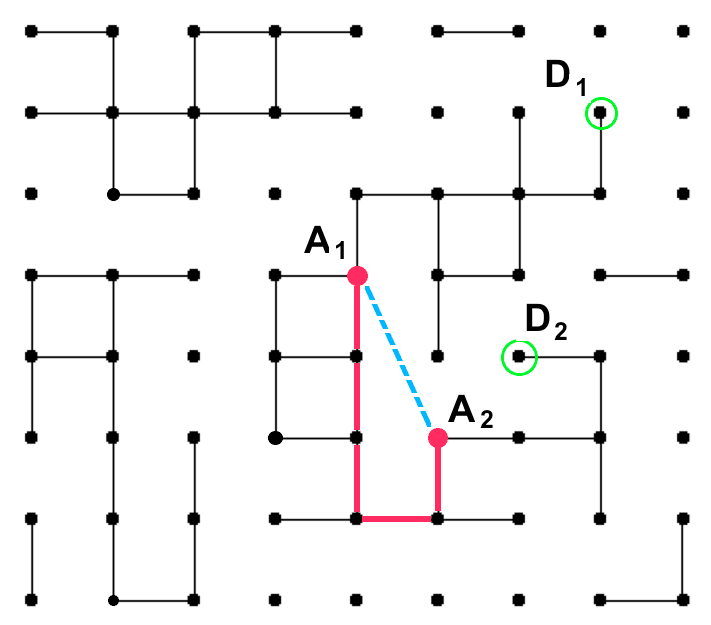
\includegraphics{figures/griddotschemdiamlabel}}
\caption{\label{fig:griddotschemdiamlabel} Illustration of the the chemical distance $l$ (in red) and the Euclidean distance (in dashed blue) between to vertices $A_1$ and $A_2$ on a Potts cluster.  Also shown is the diameter $D$ (defined by endpoints at vertices $D_1$ and $D_2$) for the same cluster.}
\end{center}
\end{figure}

\begin{figure}[h]
\begin{center}
\scalebox{.7}{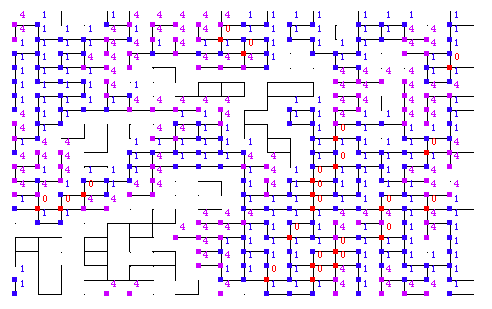
\includegraphics{figures/diamfind}}
\caption{\label{fig:diamfind} This will be a figure to go along with the quantities defined in the section on the diameter-finding algorithm.}
\end{center}
\end{figure}

\section{Bibliography}
\bibliographystyle{apsrev}
\bibliography{../bibfiles/dwbreferences}

\end{document}